% THIS IS AN EXAMPLE DOCUMENT FOR VLDB 2012
% based on ACM SIGPROC-SP.TEX VERSION 2.7
% Modified by  Gerald Weber <gerald@cs.auckland.ac.nz>
% Removed the requirement to include *bbl file in here. (AhmetSacan, Sep2012)
% Fixed the equation on page 3 to prevent line overflow. (AhmetSacan, Sep2012)

\documentclass{vldb}
\usepackage{graphicx}
\usepackage{balance}  % for  \balance command ON LAST PAGE  (only there!)
\usepackage{hyperref}       % hyperlinks
\usepackage{graphicx}
\usepackage{comment}
\usepackage{multicol}
\usepackage{framed}
\usepackage{subcaption}
\usepackage{url}            % simple URL typesetting
\usepackage{booktabs}       % professional-quality tables
\usepackage{amsfonts}       % blackboard math symbols
\usepackage{nicefrac}       % compact symbols for 1/2, etc.
\usepackage{microtype}      % microtypography
\usepackage{amsmath}

% Include information below and uncomment for camera ready
\vldbTitle{A Sample Proceedings of the VLDB Endowment Paper in LaTeX Format}
\vldbAuthors{Ben Trovato, G. K. M. Tobin, Lars Th{\sf{\o}}rv{$\ddot{\mbox{a}}$}ld, Lawrence P. Leipuner, Sean Fogarty, Charles Palmer, John Smith, Julius P.~Kumquat, and Ahmet Sacan}
\vldbDOI{https://doi.org/10.14778/xxxxxxx.xxxxxxx}
\vldbVolume{12}
\vldbNumber{xxx}
\vldbYear{2019}

\begin{document}

% ****************** TITLE ****************************************

\title{Using VDMS to Search 100M Images: A Piece of Cake}


% possible, but not really needed or used for PVLDB:
%\subtitle{[Extended Abstract]
%\titlenote{A full version of this paper is available 
% as\textit{Author's Guide to Preparing ACM SIG Proceedings Using 
% \LaTeX$2_\epsilon$\ and BibTeX} at \texttt{www.acm.org/eaddress.htm}}}

% ****************** AUTHORS **************************************

% You need the command \numberofauthors to handle the 'placement
% and alignment' of the authors beneath the title.
%
% For aesthetic reasons, we recommend 'three authors at a time'
% i.e. three 'name/affiliation blocks' be placed beneath the title.
%
% NOTE: You are NOT restricted in how many 'rows' of
% "name/affiliations" may appear. We just ask that you restrict
% the number of 'columns' to three.
%
% Because of the available 'opening page real-estate'
% we ask you to refrain from putting more than six authors
% (two rows with three columns) beneath the article title.
% More than six makes the first-page appear very cluttered indeed.
%
% Use the \alignauthor commands to handle the names
% and affiliations for an 'aesthetic maximum' of six authors.
% Add names, affiliations, addresses for
% the seventh etc. author(s) as the argument for the
% \additionalauthors command.
% These 'additional authors' will be output/set for you
% without further effort on your part as the last section in
% the body of your article BEFORE References or any Appendices.

\numberofauthors{8} %  in this sample file, there are a *total*
% of EIGHT authors. SIX appear on the 'first-page' (for formatting
% reasons) and the remaining two appear in the \additionalauthors section.

\author{
% You can go ahead and credit any number of authors here,
% e.g. one 'row of three' or two rows (consisting of one row of three
% and a second row of one, two or three).
%
% The command \alignauthor (no curly braces needed) should
% precede each author name, affiliation/snail-mail address and
% e-mail address. Additionally, tag each line of
% affiliation/address with \affaddr, and tag the
% e-mail address with \email.
%
% Authors
\alignauthor
Luis Remis\titlenote{Most of the work was done while at Intel Labs.}\\
%       \affaddr{Institute for Clarity in Documentation}\\
%       \affaddr{1932 Wallamaloo Lane}\\
       \affaddr{ApertureData Inc.}\\
       \email{luis@aperturedata.io}
\alignauthor
Chaunte Lacewell\\
%       \affaddr{Institute for Clarity in Documentation}\\
%       \affaddr{P.O. Box 1212}\\
       \affaddr{Intel Labs}\\
       \email{chaunte.w.lacewell@intel.com}
}
% There's nothing stopping you putting the seventh, eighth, etc.
% author on the opening page (as the 'third row') but we ask,
% for aesthetic reasons that you place these 'additional authors'
% in the \additional authors block, viz.
%\additionalauthors{Additional authors: John Smith (The Th{\o}rv\"{a}ld Group, {\texttt{jsmith@affiliation.org}}), Julius P.~Kumquat
%(The \raggedright{Kumquat} Consortium, {\small \texttt{jpkumquat@consortium.net}}), and Ahmet Sacan (Drexel University, {\small \texttt{ahmetdevel@gmail.com}})}
%\date{30 July 1999}
% Just remember to make sure that the TOTAL number of authors
% is the number that will appear on the first page PLUS the
% number that will appear in the \additionalauthors section.


\maketitle

\begin{abstract}
We introduce the Visual Data Management System (VDMS),
which enables faster access to big-{\em visual}-data
and adds support to visual analytics.
This is achieved by searching for relevant visual data via metadata stored as
a graph, and enabling faster access to visual data through new
machine-friendly storage formats. VDMS differs from existing large scale photo
serving, video streaming, and textual big-data management systems due to
its primary focus on supporting machine learning and
data analytics pipelines that use visual data
(images, videos, and feature vectors), treating these as first class entities.
We describe how to use VDMS via its user friendly interface and how
it enables rich and efficient vision analytics through a machine learning
pipeline for processing medical images. We show the improved
performance of 2x in complex queries over a comparable set-up.
\end{abstract}

\section{Introduction}
\label{intro}

Visual computing workloads performing analytics on
video or image data, either off-line or streaming,
have become prolific across a wide range of application domains.
This is in part due to the growing ability of machine learning (ML) techniques to
extract information from the visual data which can subsequently be used
for informed decision making \cite{vdms-nips}.
The insights this information can provide depend on the
application: a retail vendor might be interested in the amount of time
want to see the effect of a specific treatment on the size of a tumor.

Despite this rich and varied usage environment, there has been very little
research on the management of visual data.
Most of the current storage solutions for visual data are
an ad-hoc collection of tools and systems. 
For example, consider a ML developer constructing a pipeline
for extracting brain tumor information from existing brain images in a
classic medical imaging use case. 
This requires assigning consistent
identifiers for the scans and adding their metadata in
some form of relational or key-value database. 
If the queries require a search over some patient information, 
then patients have to be associated with their brain scans. 
Finally, if the ML pipeline needs images that
are of a size different than the stored ones, there is additional compute
diverted towards pre-processing after the potentially larger images are fetched. 
All these steps require investigation of different software
solutions that provide various functionalities that can then be stitched
together with a script for this specific use case.
Moreover, if the pipeline identifies
new metadata to be added for the tumor images, most databases make it
hard to evolve the schema on the fly.
As another example, many applications that can be studied through the use of large
and publicly available datasets. 
Applications include basic image search functionality (through the use
of human-generated tags), advanced image search through the use of
machine-generated tags and feature vectors\cite{imagesearch} 
for each image, and video summarization.
For these use-cases, the usual first step consists on selecting a 
subset of the data before running any processing, and a large effort 
is devoted to cleaning up and pre-processing the data.
Selecting subsets of data is by itself a time consuming task,
as it involves loading all metadata into a solution that enables searching
based on tags (relational database, graph database, csv files, etc), and
building the necessary pipelines for querying and retrieving the right data.

More generally, data scientists and machine learning developers 
usually end up building an ad-hoc solution that results in a 
combination of databases and file systems to store 
metadata and visual data (images, videos), respectively. 
This is integrated with a set of custom scripts that tie multiple systems together, 
unique not only to a specific application/discipline but often to individual researchers.
These ad-hoc solutions make replicating experiments difficult, 
and more importantly, they do not scale well when deployed in the real-world.
The reason behind such complexity is the lack of a one-system 
that can be used to store and access all the data the application needs.

In this paper, we show how VDMS~\cite{vdms-nips} provides a comprehensive solutions 
to the data management for applications that heavily rely on visual data. 
VDMS is an Open Source project designed to enable efficient access of visual data.
We also expand on the video and feature vector capabilities of
VDMS, which are part of the latest additions to the system.
We analyze different functionalities and trade-offs for this type of data,
in combination with metadata filtering. 
To the best of our knowledge, this set of functionalities, 
provided behind an integrated API, are unique to VDMS and 
we were unable to find a system with similar functionality.
We show how VDMS can be used as the single and centralize point for data
management and data access even when having multiple modalities of data:
Metadata, Image, Videos, and Feature Vectors.

For this work, we use the YFCC100M dataset\cite{Thomee_2016}. 
The YFCC100M is the largest publicly multimedia collection. 
It contains the metadata of around 99.2 million photos 
and 0.8 million videos from Flickr,
plus expansion packs that include a variety of multidimensional data,
all of which were shared under one of the various Creative Commons licenses.
We have used this dataset
for multiple proof of concepts and applications within our research lab. 

\section{VDMS Design \& Implementation}
\label{arch}

In this section, we further describe VDMS design principles and implementation,
which was briefly introduced in previous work \cite{vdms-nips}.
VDMS implementation is fully open-sourced
\footnote{https://github.com/IntelLabs/vdms}.

\begin{figure}
\centering
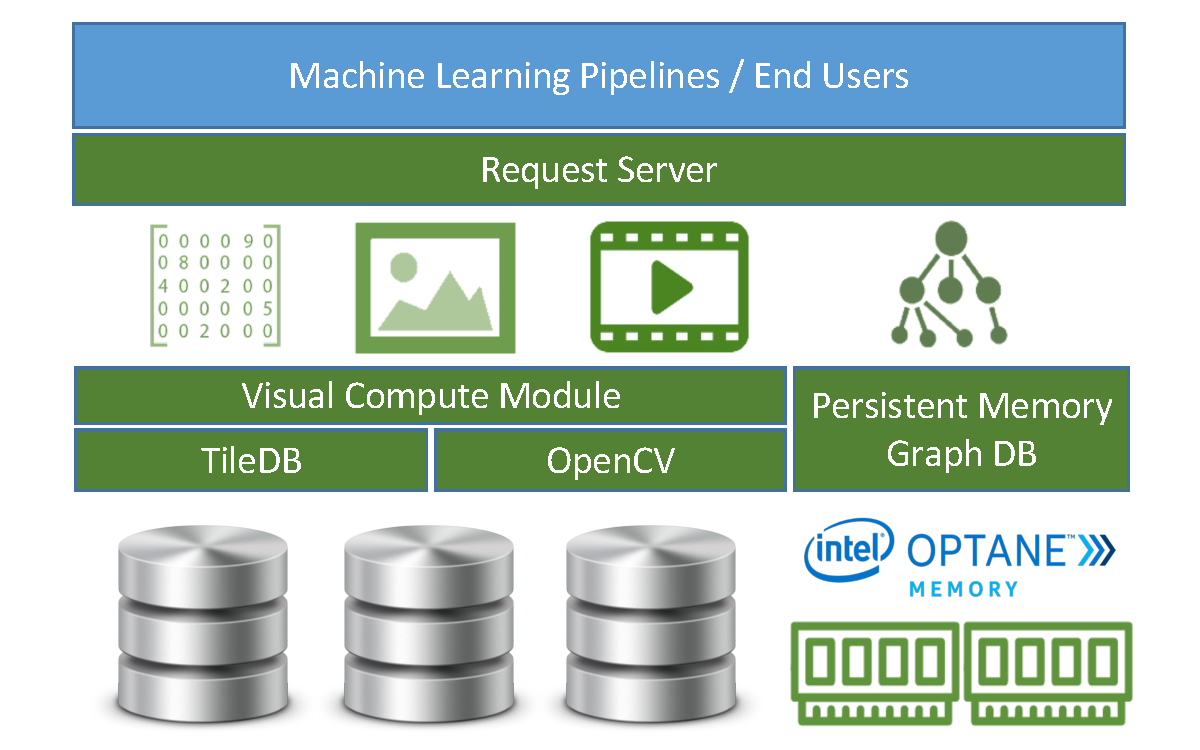
\includegraphics[width=1\columnwidth]{figures/vdms_arch.pdf}
\caption{VDMS Architecture}
\label{fig:arch}
\end{figure}

VDMS implements the typical client-server architecture that handles
client queries transactionally and concurrently, similar to what most common
relational and non-relational database systems
\cite{mysql, postgresql, chang2008bigtable} use.
The main difference between other data management systems and VDMS is that
it goes beyond the typical supported data types (string, integers, floats,
blobs, JSON-documents, etc), recognizing visual entities (image, videos,
feature vectors, etc) as first class citizens.
VDMS API enable users to insert, index, process, and query visual data,
as well as provides full support for inserting, indexing and querying
user-defined metadata.
Users interact with both metadata and visual data using a unified API,
in a transactional manner.

VDMS provides a \textit{graph model} abstraction with the traditional
atomicity, consistency, isolation, and durability
(ACID) properties expected from databases.
This is, users interact with their objects (metadata, images, videos, etc.),
as if these objects were in a connected graph.
Graph represents an easier abstraction to model complex problems,
making it very suitable for the data and access patterns shown by visual metadata,
which can be easily mapped into application-level abstractions by
developers~\cite{tao}.
For instance, abstractions like \textit{BoundingBoxes} associated to
images or videos can be easily represented using nodes and edges in a graph.
This is the main reason why the team chose a graph model over a
relational one for the implementation of VDMS API.

VDMS API provides a mechanism to insert and connect Images, Videos, BoundingBoxes,
Frames, and Descriptors (feature vectors), together with any metadata
associated with the objects.
Each object is a node in the graph.
The information associated to each visual object (image, video, etc.) is modeled as
"properties" of the node in the graph.
Users can query, filter, and retrieve these objects based on its properties.
VDMS does not simply treat these objects as binary blobs of data, but rather
understands them and the type of processing that is common for them,
providing the ability to run processing on-the-fly, both at insertion and
retrieval time. This is one of the main differentiating aspects when compared to other
database systems, including relational databases.
In a relational database, for instance, one can query \textit{and compute}
over values in a column only for basic data types (strings, integers, floats),
and over the abstractions the relational model supports (tables, columns).
This is, a SQL query can retrieve the \textit{computed average} "salary" of all
the employees in a company (stored using the table/columns abstraction),
but cannot perform any computation over data stored as a blob or binary object.
VDMS, because it recognized the nature of visual objects by design,
provides the ability to \textit{compute} on these visual objects
(image, videos, etc.).

VDMS API also allows users to insert application-defined "Entities",
that enable applications to model any use-case specific metadata.
An "Entity" object (and its properties) is a node in the graph.
For example, a user can define an Entity object of a class "Person",
and \textit{connect} this person to one or multiple image objects.
Later, the user can retrieve the Entity object corresponding to a person,
together with all the images \textit{connected} to it. In some cases,
users may need to apply different processing operations to the visual data
for their application. We chose to support
specific operations due to their frequent use in ML applications using
visual data. Common operations supported for both images and videos are
thresholding, cropping, and resizing. Additional operations such as
flipping and rotation are supported for images and extracting
frames by interval is supported for videos.
In most ML applications, a subset of these operations are included in
the preprocessing stage of model training and/or inferencing which supports
majority of the research communities who analyze visual data and may benefit
from replacing customized solutions with VDMS.

By providing the ability to store visual data objects together with
application-defined entities and its properties, VDMS can manage
all the data the application need behind a single, unified API.
This means users can access all data (metadata, images, videos, etc.)
from the VDMS API and even implement their own API/front-end on top
of VDMS without adding any additional abstractions.
This is in contrast with current applications that rely on a combination
of multiple data management systems and APIs to access different
portions of the data they need
\cite{tao, sculley2015hidden, mayer2020scalable, sculley2015hidden}.

Figure \ref{fig:arch} depicts the high-level architecture of VDMS, which
is composed by several sub-components, and a Query Engine that implements
the unified API and hides all the complexity underneath.
We first describe the VDMS API, and then describe its sub-components
and design decisions.

\subsection{VDMS API}

One of the most important differentiating aspects of VDMS is its API.
VDMS is unique in recognizing visual entities (i.e., images, videos, etc.)
as first class citizens.
Thus, VDMS' API revolves around visual data operations and retrieval,
but at the same time, enables applications to store any other
application-specific metadata.
VDMS API is easy to use and explicitly pre-defines certain
primitives associated with metadata, images, videos, and feature vectors.
Authors have paid particular attention to hide the complexities of our internal
implementation and up-level the API to a JSON-based API,
which is very popular across various application domains.
By defining a new JSON-based API, there is a trade-off between expressiveness
(compared to well-established query languages like SPARQL, Gremlim, or even SQL)
and the ability to natively support visual data operations.
However, we believe it is possible for our API to achieve similar levels of
expressiveness compared to more mature query languages over time.

Listing~\ref{addimageandautotag} shows a sample query for inserting
an image, properties associated with the image, and metadata to VDMS.
The metadata, in this case, is the information about the "autotag",
which is provided by the dataset in this specific
\textit{image-search} application.
In this example, the transaction inserts an application-defined "Entity" of
the class "autotag", with the "name" property being \textit{alligator},
inserts an Image with its "latitude" and "longitude",
stores the image as a JPG (VDMS will transcode if needed),
and creates a connection between the Image and the Entity, with a "prob"
property (which indicates the probability of that image
containing an object of type  \textit{alligator}) with a specific value.
This query is performed \textit{transactionally}: either all the image, metadata
and connection are inserted, or none of them are and an error is returned.
Note that no schema needs to be defined in advance.
The Entity of class "autotag", with its properties, are declared and added
at insertion time, without any need to define a schema of objects
(and its properties) before hand. This is a benefit over relational
databases which require the user to identify how data is divided into
different tables and determine the relationship between tables.

\begin{listing}[ht!]
\begin{minted}[frame=single,
              framesep=3mm,
              linenos=true,
              xleftmargin=21pt,
              fontsize=\footnotesize,
              tabsize=4]{js}
"AddEntity"{
    "_ref" : 1,
    "class": "autotag",
    "properties": {
        "name": "alligator"
    }
},
"AddImage":{
    "_ref": 2,
    "properties": {
        "latitude":    36.23433,
        "longitude": -116.80666
    },
    "format": "jpg"
},
"AddConnection": {
    "ref1": 1,
    "ref2": 2,
    "properties": {
        "prob": 0.7653
    }
}

\end{minted}
\caption{Sample Query for Image Insertion -
The query expresses the following:
Insert an Entity of the class "autotag", with the "name" property being
\textit{alligator}, insert an Image with its "latitude" and "longitude",
store the image as a JPG, and create a connection between
the image and the "autotag", with a property "prob"
(which indicates the probability of that image
containing an object of type \textit{alligator}).}
\label{addimageandautotag}
\end{listing}

Listing~\ref{findimagegeo} shows another sample query, in this case, for retrieval.
In this particular example, the transaction retrieves all the images
of \textit{alligators} with probability higher than 0.66,
filter by latitude and longitude within 1 degree,
apply a resize operation to make the images 224x224,
rotate the images 45.34 degrees, and return the images as "png" files.
It is important to note how the API natively supports basic building
blocks of visual data processing, like resize, rotation, or transcoding
(changing output formats and encodings).
Moreover, because VDMS is in control of the metadata and the image data,
re-ordering or pre-processing operations can be done transparently,
increasing the performance of the retrieval process.
The API allows interaction with metadata, images, videos, bounding boxes,
frames, feature vectors, and more in a similar fashion,
and it is fully documented on the project's Github
wiki~\footnote{https://github.com/IntelLabs/vdms/wiki/API-Description}.
The visual data pre-processing operations supported in VDMS are generic and
application independent.
By design, we only include pre-processing operations that are not specific
to one domain, but rather general for visual analytics.



\begin{listing}[ht!]
\begin{minted}[frame=single,
              framesep=3mm,
              linenos=true,
              xleftmargin=21pt,
              fontsize=\footnotesize,
              tabsize=4]{js}
"FindEntity"{
    "_ref" : 1,
    "class": "autotag",
    "constraints": {
        "name": ["==", "alligator"]
    }
},
"FindImage":{
    "format": "png",
    "constraints": {
        "latitude": [">=", 36.23433,
                     "<=", 38.23433]
        "longitude":[">=", -114.80666,
                     "<=", -116.80666]
    },
    "operations": [{
            "type": "resize",
            "height": 224,
            "width":  224,
        }, {
            "type": "rotate",
            "angle": 45.34
    }],
    "link": {
        "ref":1,
        "constraints": {
            "prob": [">=", 0.66]
        }
    }
}

\end{minted}
\caption{Sample Query for Image Retrieval -
The query expresses the following:
Find all the images connected to the autotag \textit{alligator}
with probability higher than 0.66,
filter the images by latitude and longitude within 1 degree,
apply a resize operation to make the images 224x224,
rotate the image 45.34 degrees,
and return the images as "png" files.}
\label{findimagegeo}
\end{listing}

\subsection{Graph Engine}

The Graph Engine used in VDMS is the
\textit{Persistent Memory Graph Database} (PMGD).
PMGD was developed at Intel Labs, and was designed and optimized for
persistent memory technologies like Intel Optane~\cite{IntelXPoint15}, which
promise storage providing nearly the speed of DRAM and the
durability of block-oriented storage.
PMGD is also fully open-sourced \footnote{https://github.com/IntelLabs/pmgd}.
PMGD implements an in-persistent-memory graph database optimized
to run on a platform equipped with persistent memory, but
also provides the option to run on SSD and ext4 filesystem
using OS support to provide transactional guarantees (through \textit{msync}).
PMGD provides a property graph model of data storage with the traditional
atomicity, consistency, isolation, and durability
(ACID) properties expected from databases.
Specifically, the database remains consistent, each transaction either
completes entirely or not at all, and the effects of a completed transaction
survives any failure.
In cases where the system may crash or fail, PMGD has the ability
to recover to a consistent state without loading its content into memory.
Unlike existing graph databases that are disk-based, our graph engine
avoids converting data from a disk-friendly format to an usable format for an application.
PMGD comes as a C++ library that VDMS uses for implementing its query engine.
Because PMGD already supports most of the graph abstractions we wanted
to see on VDMS API, it was our preferred option.
Also, our internal evaluation shows that PMGD is faster
than other graph databases, including Neo4j\cite{miller2013graph}.
In this paper, the evaluation uses SSDs instead of persistent memory.
Hence, PMGD performance evaluation will be published separately to highlight
the advantages of using persistent memory for visual data.

\subsection{Visual Compute Module}

% The Visual Compute Module enables machine-friendly enhancements to
% visual data, exposing high-level abstractions to the \textit{Request Server}
% for dealing with a variety of images and video formats (through OpenCV and ffmpeg),
% and different methods for indexing for feature vectors
% (including Facebook's Faiss \cite{faiss}, TileDB \cite{TileDB}).
% Finally, a main component of VDMS is in charge of implementing the
% API and orchestrating between the PMGD and the Visual Compute Module
% to serve client's requests. This component is the \textit{Request Server}.

The Visual Compute Module was designed and implemented to provide
an internal abstraction layer for interacting with visual data.
It enables the query engines to coordinate and perform
visual data handling and processing
(i.e., basic building block operations like crop, resize, etc. for images/videos
and k-nearest neighbor search for feature vectors),
shown in Figure \ref{fig:arch}.
For traditional formats (jpg, png, tiff, mp4, etc.),
the interface is an abstraction layer over OpenCV.
However, it also provides a way to use novel formats that are
better suited for visual analytics: a novel, array-based lossless image format.
This format is built on the array data manager TileDB~\cite{TileDB} and
is well suited for images that are used in visual analytics.
Note that, even if VDMS currently provides support for array-based lossless
image format, we do not use it as part of this evaluation.
This work focuses on a more direct comparison with a combination of alternatives,
and thus we use the traditional format (jpg and png).
The performance comparison between the array-based lossless image format
we developed and other similar formats (like png or tiff) are outside of the
scope of this evaluation.

VDMS also provides full support for video storage and operations,
in a similar way it does for images.
This includes support for encoding, decoding, and transcoding of
\textit{mp4}, \textit{avi}, and \textit{mov} containers,
as well as support for \textit{xvid}, \textit{H.263} and \textit{H.264} encoders.
This is supported through the use of either OpenCV~\cite{opencv}
or \textit{libffmpeg}\cite{ffmpeg}, or both,
plus additional implementation to support fast random access to video frames.
All operations supported for images in VDMS are also supported at the
video and frame level of the API.
On top of that, there are a number of video-specific operations that
are supported, such as the interval operations,
enabling users to retrieve clips at different
frames-per-second (fps) versions of the video.

Another key differentiating factor of VDMS is that it allows the creation of
indexes for high-dimensional feature vectors and the insertion of
these feature vectors associated with entities, images, and/or videos.
Feature vectors are intermediate results of various machine
learning or computer vision algorithms when run on visual data.
Feature vectors are also known as \textit{descriptors}
or \textit{visual descriptors}.
We use these terms interchangeably.
These descriptors can be classified, labeled, and used to build search indexes.
Feature Vectors support is provided through our implementation based
on high-dimensional sparse arrays, also using array-based approaches.
In addition, the Visual Compute Library provides a wrapper
for another high-dimensional index implementation,
Facebook's Faiss~\cite{faiss}.
Users can, through our API, use different indexing techniques
for feature vectors, depending on their application's need.


\subsection{Client Library}

The client library implements TCP/IP based connectors to the VDMS Server,
similar to most databases\cite{memsql, mysql, postgresql}.
Users can connect to VDMS and run queries using VDMS' API
by defining a transaction using JSON objects.
The client library provides a simple method that
accepts a JSON string and an array or vector of blobs.
Internally, the library wraps the query string and blobs using
Google Protobufs \cite{protobufs} and sends it to the VDMS server.
It also receives a similarly formed response from VDMS
and returns it to the client.
Currently, client libraries are implemented for Python and C++ client.
The client libraries are lightweight, as they simply implement the communication
protocol between the client and the server.
This makes it easier for developers to implement similar client libraries using
any other programming language of their choice.

%\input{demo.tex}
%\section{Conclusion}
In this paper, we described VDMS design and implementation and
show a comprehensive evaluation on our Image Search Application.
We use one of the largest publicly available datasets:
The Yahoo Flickr Creative Commons 100M (YFCC100M),
together with the expansions packs that include
machine-generated labels.
We show how VDMS compares against a combination of
industry standard systems, all of which are needed to
replicate only a portion of VDMS' functionality.
We see improvements up to 364x in certain queries,
and an average improvement of about 85x when compared to PostgreSQL+Apache.
When compared to MySQL+Apache, we see up to 96x speedup
and and average improvement of 31x.
The design of VDMS, which was conceived as a
data management system that treats visual entities
as first class citizens, can remove inefficiencies
that result from re-purposing and combining solutions
that were not designed for the job while providing
simpler and richer interfaces.
VDMS' easy-to-use interfaces outperform industry standard systems
with a set of functionalities which, to the best of our knowledge,
are not available in any other single data management solution for visual data.
VDMS was designed for analytics and it can efficiently handle complex queries
which can simplify the design of future applications that rely on visual data.


% \balance

% The following two commands are all you need in the
% initial runs of your .tex file to
% produce the bibliography for the citations in your paper.
\bibliographystyle{abbrv}
\bibliography{vdms-vldb2020}
% vldb_sample.bib is the name of the Bibliography in this case
% You must have a proper ".bib" file
%  and remember to run:
% latex bibtex latex latex
% to resolve all references

\begin{framed}
\scriptsize

\noindent \textbf{Notices \& Disclaimers}

\noindent Intel technologies may require enabled hardware, software or service activation.

\noindent No product or component can be absolutely secure.

\noindent Your costs and results may vary. 

\noindent \copyright Intel Corporation.  Intel, the Intel logo, and other Intel marks are trademarks of Intel Corporation or its subsidiaries.  Other names and brands may be claimed as the property of others. 

\noindent Intel does not control or audit third-party data.  You should consult other sources to evaluate accuracy.

\noindent Intel disclaims all express and implied warranties, including without limitation, the implied warranties of merchantability, fitness for a particular purpose, and non-infringement, as well as any warranty arising from course of performance, course of dealing, or usage in trade.

% \copyright  Intel Corporation.  Intel, the Intel logo, and other Intel marks are trademarks of Intel Corporation or its subsidiaries.  Other names and brands may be claimed as the property of others.

% Performance results are based on testing as of dates shown in configurations and may not reflect all publicly available security updates.  See backup for configuration details.  No product or component can be absolutely secure.

% Your costs and results may vary.

% Intel technologies may require enabled hardware, software or service activation.

% Software and workloads used in performance tests may have been optimized for performance only on Intel microprocessors.  Performance tests, such as SYSmark and MobileMark, are measured using specific computer systems, components, software, operations and functions.  Any change to any of those factors may cause the results to vary.  You should consult other information and performance tests to assist you in fully evaluating your contemplated purchases, including the performance of that product when combined with other products.   For more complete information visit www.intel.com/benchmarks.

% Intel's compilers may or may not optimize to the same degree for non-Intel microprocessors for optimizations that are not unique to Intel microprocessors. These optimizations include SSE2, SSE3, and SSSE3 instruction sets and other optimizations. Intel does not guarantee the availability, functionality, or effectiveness of any optimization on microprocessors not manufactured by Intel. Microprocessor-dependent optimizations in this product are intended for use with Intel microprocessors. Certain optimizations not specific to Intel microarchitecture are reserved for Intel microprocessors. Please refer to the applicable product User and Reference Guides for more information regarding the specific instruction sets covered by this notice.  Notice Revision \#20110804
\end{framed}


\subsection{References}
Generated by bibtex from your ~.bib file.  Run latex,
then bibtex, then latex twice (to resolve references).

%APPENDIX is optional.
% ****************** APPENDIX **************************************
% Example of an appendix; typically would start on a new page
%pagebreak

\begin{appendix}
You can use an appendix for optional proofs or details of your evaluation which are not absolutely necessary to the core understanding of your paper. 

\section{Final Thoughts on Good Layout}
Please use readable font sizes in the figures and graphs. Avoid tempering with the correct border values, and the spacing (and format) of both text and captions of the PVLDB format (e.g. captions are bold).

At the end, please check for an overall pleasant layout, e.g. by ensuring a readable and logical positioning of any floating figures and tables. Please also check for any line overflows, which are only allowed in extraordinary circumstances (such as wide formulas or URLs where a line wrap would be counterintuitive).

Use the \texttt{balance} package together with a \texttt{\char'134 balance} command at the end of your document to ensure that the last page has balanced (i.e. same length) columns.

\end{appendix}



\end{document}
